\documentclass{standalone}
\usepackage{tikz}
\usetikzlibrary{decorations.pathreplacing}
\usepackage{amsfonts}

\begin{document}
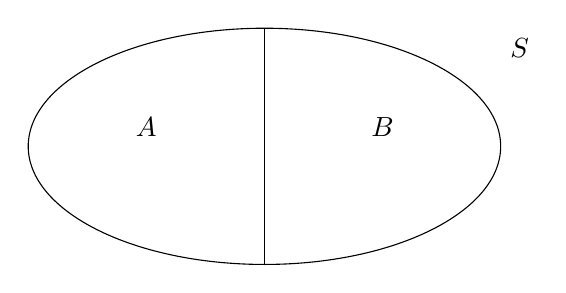
\begin{tikzpicture}
  % Define the set S as an ellipse
  \draw (0,0) ellipse (3cm and 1.5cm);
  
  % Label the parts A and B
  \node at (-1.5, 0.25) {$A$};
  \node at (1.5, 0.25) {$B$};
  
  % Label for set S outside the ellipse
  \node[above right] at (3, 1) {$S$};
  
  % Divide the ellipse into two equal parts with a vertical line
  \draw (0,1.5) -- (0,-1.5);
 \end{tikzpicture}
\end{document}